\documentclass[12pt]{article}

\usepackage[margin=1in]{geometry}
\usepackage{amsmath,amsthm,amssymb}
\usepackage{float}
\usepackage{graphicx}
\usepackage{bbold}
\usepackage{algorithm}
\usepackage{algcompatible}
\usepackage{csquotes}
\usepackage{url}

\newcommand{\N}{\mathbb{N}}
\newcommand{\Z}{\mathbb{Z}}
\newcommand{\abs}[1]{\left| #1 \right|}
\newcommand{\norm}[1]{\left|\left| #1 \right|\right|}
\newcommand{\ceil}[1]{\left\lceil #1 \right\rceil}
\newcommand{\floor}[1]{\left\lfloor #1 \right\rfloor}
\newcommand{\pprime}{\prime \prime}
\newcommand{\BigO}[1]{\mathcal{O}\left( #1 \right)}
\newcommand{\proj}[2][]{\textit{proj}_{\vect{#1}}\vect{#2}}
\newcommand{\vect}{\mathbf}
\newcommand{\Id}{\mathbb{1}}
\newcommand{\inv}[1]{ #1^{-1}}
\newcommand{\minn}{\text{min}}
\newcommand{\maxx}{\text{max}}
\renewcommand{\P}[1]{\left( #1 \right)}
\newcommand{\diag}[1]{\text{diag}\P{#1}}
\newcommand{\grad}{\nabla}
\newcommand{\laplacian}{\nabla^{2}}

\newenvironment{theorem}[2][Theorem]{\begin{trivlist}
\item[\hskip \labelsep {\bfseries #1}\hskip \labelsep {\bfseries #2.}]}{\end{trivlist}}
\newenvironment{lemma}[2][Lemma]{\begin{trivlist}
\item[\hskip \labelsep {\bfseries #1}\hskip \labelsep {\bfseries #2.}]}{\end{trivlist}}
\newenvironment{exercise}[2][Exercise]{\begin{trivlist}
\item[\hskip \labelsep {\bfseries #1}\hskip \labelsep {\bfseries #2.}]}{\end{trivlist}}
\newenvironment{problem}[2][Problem]{\begin{trivlist}
\item[\hskip \labelsep {\bfseries #1}\hskip \labelsep {\bfseries #2.}]}{\end{trivlist}}
\newenvironment{question}[2][Question]{\begin{trivlist}
\item[\hskip \labelsep {\bfseries #1}\hskip \labelsep {\bfseries #2.}]}{\end{trivlist}}
\newenvironment{corollary}[2][Corollary]{\begin{trivlist}
\item[\hskip \labelsep {\bfseries #1}\hskip \labelsep {\bfseries #2.}]}{\end{trivlist}}

\renewcommand{\algorithmicrequire}{\textbf{Input:}}
\renewcommand{\algorithmicensure}{\textbf{Output:}}

\DeclareMathOperator{\sech}{sech}
\DeclareMathOperator{\csch}{csch}

\begin{document}

\title{CS6210: Homework 5}
\author{Christopher Mertin}
\date{November 22, 2016}
\maketitle

\begin{enumerate}
%%%%%% Problem 1 %%%%%%
\item An $n \times n$ linear system of equations $A\vect{x} = \vect{b}$ is modified
in the following manner: For each $i = \{1,\ldots,n\}$, the value $b_{i}$ on
the right-hand side of the $i^{th}$ equation is replaced by $b_{i} - x_{i}^{3}$.
Obviously, the modified system of equations (for the unknowns $x_{i}$) is now nonlinear.

\begin{enumerate}
  \item Find the corresponding Jacobian Matrix

  {\bf Solution:}

  After making the nonlinearity change, each row in the linear system
  has the following format:

  \begin{align*}
    a_{i,1}x_{1} + \cdots + a_{i,n}x_{n} &= b_{i} - x_{i}^{3}
    \intertext{Where we can add a vector of $\vect{x}^{3}$ (denoting the cubing of each element independently) to each side, giving}
    a_{i,1}x_{1} + \cdots + \left( a_{i,i}x_{i} + x_{i}^{3}\right) + \cdots + a_{i,n}x_{n} &= b_{i}
  \end{align*}

  Giving the Jacobian of $A$ as being

  \begin{align*}
    J[A] &= \begin{pmatrix}
            a_{1,1} + 3x_{1}^{2} & a_{1,2} & \cdots & a_{1,n}\\
            a_{2,1} & a_{2,2} + 3x_{2}^{2} & \cdots & a_{2,n}\\
            \vdots & \vdots & \ddots & \vdots\\
            a_{n,1} & a_{n,2} & \cdots & a_{n,n} + 3x_{n}^{2}
            \end{pmatrix}
  \end{align*}

  \item Given that $A$ is strictly diagonally dominant with positive elements on
  its diagonal, state whether or not it is guarenteed that the Jacobian matrix at
  each iterate is nonsingular.

  {\bf Solution:}

  We can look at the matrix $J^{\prime}$ to determine this, with
  $J = J^{\prime} = A + \text{diag}\P{3x_{i}^{2}}$, with $A$ being the coefficient matrix
  and the diagonal matrix being the nonlinear elements added to $J$ along the
  diagonal.

  As $A$ is diagonally dominant, and since the off-diagonals of $\text{diag}\P{3x_{i}^{2}}$
  are zero, making it diagonally dominant as well, we can say that $J^{\prime}$ (and $J$)
  are also diagonally dominant since the sum of two diagonally dominant matrices are
  diagonally dominant themselves. There is also a theorem which guarentees that every
  diagonally dominant matrix is non-singular, meaning that $J$
  is guarenteed to be non-singular.

  \item Suppose that $A$ is symmetric positive definition (not necessarily
  diagonally dominant) and that Newton's method is applied to solve the nonlinear
  system. Is it guarenteed to converge?

  {\bf Solution:}

  The definition of a matrix to be symmetric positive definite, then with $\vect{z}$
  being a positive vector, we should get
  \begin{align*}
  \vect{z}^{T}J\vect{z} &= \vect{z}^{T}\left( A + \diag{3x_{i}^{2}}\right)\\
   &= \vect{z}^{T}A\vect{z} + \vect{z}^{T}\diag{3x_{i}^{2}}\vect{z}
  \end{align*}

  with $\vect{z}^{T}A\vect{z}$ being positive since $A$ is symmetric positive definite.
  $\diag{3x_{i}^{2}}$ is always positive along the diagonal, so $\vect{z}^{T}\diag{3x_{i}^{2}}\vect{z}$
  is also always positive, and symmetric (due to the off diagonals being zero). Therefore,
  $J$ is symmetric positive definite and Newton's Method will converge.
\end{enumerate}

%%%%%% Problem 2 %%%%%%
\item \

\begin{enumerate}
  \item Suppose Newton's method is applied to a linear system $A\vect{x} = \vect{b}$.
  How does the iterative formula look and how many iterations does it take to converge?

  {\bf Solution:}

  The equation for Newton's Method is
  \begin{align*}
    J[\vect{x}]p_{k} &= -f(\vect{x})\\
    \intertext{So we have to calculate the Jacobian of $f(x) = A\vect{x} - \vect{b}$, which is $J[\vect{x}] = A$, giving}
    Ap_{k} &= -f(\vect{x})\\
    \intertext{with a given $\vect{x}_{0}$ of an initial guess, it gives}
    Ap_{0} &= -\left( A\vect{x}_{0} - \vect{b}\right)\\
    \intertext{Where we can multiply by the interverse of $A$, giving}
    p_{0} &= -\vect{x}_{0} + \inv{A}\vect{b}
    \intertext{where we can finally show that it will require only one iteration for convergence}
    \vect{x}_{1} &= \vect{x}_{0} + p_{0} = \vect{x}_{0} + \left( -\vect{x}_{0} + \inv{A}\vect{b}\right) = \inv{A}\vect{b}
  \end{align*}

  \item Suppose the Jacobian matrix is singular at the solution of a nonlinear system
  of equations. Speculate what can occur in terms of convergence and the rate of convergence.
  Specifically, is it possible to have a situation where the newton iteration converges but
  convergence is not quadratic?

  {\bf Solution:}

  The text states that the Jacobian matrix should have a bounded inverse and also
  a continuous derivative to guarentee that Newton's Method can converge quadratically.
  However, the question states that the Jacobian is singular, so it won't converge
  quadratically.

\end{enumerate}

%%%%%% Problem 3 %%%%%%
\item Consider minimizing the function $\phi(\vect{x}) = \vect{c}^{T}\vect{x} + \frac{1}{2}\vect{x}^{T}H\vect{x}$,
where $\vect{c} = \left( 5.04,-59.4,146.4,-96.6\right)^{T}$ and

\[
  H = \begin{pmatrix}0.16 & -1.2 & 2.4 & -1.4 \\
                     -1.2 & 12.0 & -27.0 & 16.8\\
                     2.4  & -27.0 & 64.8 & -42.0\\
                     -1.4 & 16.8 & -42.0 & 28.0\end{pmatrix}
\]

Try both Newton and BFGS methods, starting from $\vect{x}_{0} = \left( -1,3,3,0\right)^{T}$.
Explain why the BFGS method requires significantly more iterations than Newton's.

{\bf Solution:}

\begin{itemize}
  \item {\sc Broyden-Fletcher-Goldfarb-Shanno (BFGS)}

  The necessary condition for minimization at $\widetilde{\vect{x}}$ is $\grad\phi\P{\widetilde{\vect{x}}} = 0$,
  so in finding $\grad\phi(\vect{x})$
  \begin{align*}
    \phi(\vect{x}) &= \vect{c}^{T}\vect{x} + \frac{1}{2}\vect{x}^{T}H\vect{x}\\
    \grad\phi(\vect{x}) &= H\vect{x} + \vect{c}\\
    \intertext{By setting $\grad\phi(\vect{x}) = 0$}
    H\vect{x} + \vect{c} &= 0\\
    \vect{x} &= -\inv{H}\vect{c} = \begin{pmatrix}2212.33\\ 2119.56\\ 1912.67\\ 1711.33\end{pmatrix}
  \end{align*}
  \item {\sc Newton}

  For Newton's Method, the requirement is

  \begin{align*}
    \laplacian\phi(\vect{x}_{k})p_{k} &= -\grad\phi(\vect{x}_{k})\\
    \vect{x}_{k+1} &= \vect{x}_{k} + p_{k}\\
    \intertext{So, in solving for $\laplacian\phi$}
    \grad\phi(\vect{x}) &= H\vect{x} + \vect{c}\\
    \laplacian\phi(\vect{x}) &= H
    \intertext{And in solving for $p_{k}$}
    p_{k} &= -\inv{\P{\laplacian\phi(\vect{x}_{k})}}\grad\phi(\vect{x}_{k})\\
          &= -\inv{H}\P{H\vect{x}_{k} + \vect{c}} = -\vect{x}_{k} - \inv{H}\vect{c}
   \intertext{Giving us $\vect{x}_{k+1}$ as being}
   \vect{x}_{k+1} &= \vect{x}_{k} - \vect{x}_{k} - \inv{H}\vect{c}\\
                  &= -\inv{H}\vect{c}
  \end{align*}
\end{itemize}

So the initial guess was independent of the convergence. Newton's Method is faster
at converging than {\sc BFGS} since it uses the second derivative. In the given question,
the second derivative is independent of $x$, and would thus only need one iteration.


%%%%%% Problem 4 %%%%%%
\item With the notation of Exercise 21, for $p = 2$ the problem can be solved as
in Example 9.15 using SVD. But it can also be solved using the techniques of
constrained optimization:

\begin{enumerate}
  \item Explain why it is justified to replace the objective function by $\frac{1}{2}\norm{y}_{2}^{2}$.

  {\bf Solution:}

  Multiplying a function by a constant will not change the minimization problem, just
  the final value will be shifted by that multiplicative factor.

  \item Form the KKT conditions of the resulting constrained optimization problem,
  obtaining a linear system of equations.

  {\bf Solution:}

  The conditions for KKT in the constrained minimization problem are

  \begin{align*}
    1 - \grad_{y}L\left( \widetilde{y}, \widetilde{\lambda}\right) &= 0\\
    2 - C_{i}\P{\widetilde{y}} &= 0\\
    3 - \widetilde{\lambda_{i}}C_{i}\P{\widetilde{y}} &= \grad\phi(y)
  \end{align*}

  for every Lagrangian Multiplier $\widetilde{\lambda_{i}}$.

  \item Devise an example and solve it using the method developed as well as the one
  from Example 9.15. Compare and discuss.

  {\bf Solution:}

\end{enumerate}

%%%%%% Problem 5 %%%%%%
\item Given the four data points $(-1, 1), (0,1), (1,2), (2,0)$, determine the
interpolating cubic polynomial

\begin{itemize}
  \item Using the Monomial basis
  \item Using the Lagrange basis
  \item Using the Newton basis
\end{itemize}

Show that the three representations give the same polynomial.

{\bf Solution:}

\begin{itemize}
  \item {\sc Monomial Basis}

  We should use a polynomial interpolant of degree 4, of the form

  \begin{align*}
    p(x) &= c_{0} + c_{1}x + c_{2}x^{2} + c_{3}x^{3}
    \intertext{Where we can start by putting the points in $p(x)$, giving}
    1 &= c_{0} - c_{1} - c_{2} - c_{3}\\
    1 &= c_{0}\\
    2 &= c_{0} + c_{1} + c_{2} + c_{3}\\
    0 &= c_{0} + 2c_{1} + 4c_{2} + 8c_{3}\\
    \intertext{where solving this system of equations gives}
    c_{0} &= 1\\
    c_{1} &= \frac{7}{6}\\
    c_{2} &= \frac{1}{2}\\
    c_{3} &= -\frac{2}{3}\\
    \intertext{where putting it back in $p(x)$ gives}
    p(x) &= 1 + \frac{7}{6}x + \frac{1}{2}x^{2} - \frac{2}{3}x^{3}
  \end{align*}

  \item {\sc Lagrange Basis}
  The Lagrange Interpolant is

  \begin{align*}
    p(x) &= \sum_{j=0}^{n}y_{j}L_{j}(x)\\
    \intertext{and the Lagrange Polynomials being}
    L_{j}(x) &= \prod_{i=0}^{n}\frac{x - x_{i}}{x_{j} - x_{i}}\\
    \intertext{for $i\neq j$, so solving for the polynomials gives}
    L_{0}(x) &= \frac{x(x+1)(x-2)}{(-1-0)(-1-1)(-1-2)} = -\frac{x(x+1)(x-2)}{6}\\
    L_{1}(x) &= \frac{(x+1)(x-1)(x-2)}{1(-1)(-2)} = \frac{(x+1)(x-1)(x-2)}{2}\\
    L_{2}(x) &= \frac{(x+1)x(x-2)}{(1+1)1(1-2)} = -\frac{(x+1)x(x-2)}{2}\\
    L_{3}(x) &= \frac{(x+1)x(x-1)}{(2+1)2(2-1)} = \frac{(x+1)x(x-1)}{6}\\
    \intertext{and plugging back into $p(x)$ gives}
    p(x) &= L_{0}(x) + L_{1}(x) + 2L_{3}(x) + 0\\
         &= 1 + \frac{7}{6}x + \frac{1}{2}x^{2} - \frac{2}{3}x^{3}
  \end{align*}

  \item {\sc Newton Basis}

  The Newton Interpolant is

  \begin{align*}
    p(x) &= \sum_{j=0}^{3}c_{j}\prod_{i=0}^{j-1}\P{x - x_{j}}\\
    p(x) &= c_{0} + c_{1}(x + 1) + c_{2}(x+1)x + c_{3}(x+1)x(x-1)\\
    \intertext{Where we can input the points}
    p(-1) &= c_{0} = 1\\
    p(0) &= c_{0} + c_{1} = 1\\
    p(1) &= c_{0} + 2c_{1} + 2c_{2} = 2\\
    p(2) &= c_{0} + 3c_{1} + 6c_{2} + 6c_{3} = 0\\
    \intertext{And after solving this system of equations gives}
    p(x) &= 1 + \frac{7}{6}x + \frac{1}{2}x^{2} - \frac{2}{3}x^{3}
  \end{align*}
\end{itemize}


%%%%%% Problem 6 %%%%%%
\item Suppose we are given 137 uniformly spaced data pairs at distinct abscissae:
$\left( x_{i}, y_{i}\right),i = \{ 0,1,\ldots,136\}$. These data are thought to represent
a function which is piecewise smooth; that is, the unknown function $f(x)$ which
gave rise to these data values has many bounded derivatives everywhere expect for
a few points where it jups discontinuously. (Imagine drawing a curve smoothly from
left to right, mixed with lifting the pen and moving it vertically a few times.)
For each sub interval $[x_{i-1},x_{i}]$ we wanit to pass the hopefully best cubic
$p_{3}(x)$ for an accurate interpolation of $f(x)$ at points $x_{i-1}<x<x_{i}$.
This involves choosing good neighbors to interpolate at.

Propose an algorithm for this task. Justify.

{\bf Solution:}

A cubic interpolation requires four points for each subinterval. Two of the points
are trivial and can be used as the end points. The other two we can choose neighbor
points of the subinterval endpoints.

\begin{algorithm}[H]
\begin{algorithmic}[1]
\IF{Sub Interval is $\P{x_{0},x_{1}}$}
    \STATE{Find a cubic interpolation by using $\{ x_{0},x_{1},x_{2},x_{3}\}$}
\ELSIF{Sub Interval is $\P{x_{i}, x_{i+1}}$}
    \STATE{Find a cubic interpolation by using $\{ x_{i-1}, x_{i}, x_{i+1}, x_{i+2}\}$}
\ELSIF{Sub Interval is $\P{x_{n-2}, x_{n-1}}$}
    \STATE{Find a cubic interpolation by using $\{ x_{n-4}, x_{n-3}, x_{n-2}, x_{n-1}\}$}
\ENDIF
\end{algorithmic}
\end{algorithm}

Since we are using the exact values of $\P{x_{i}, y_{i}}$, it should give an ``accurate''
interpolation as the question asked. If we wanted an approximation, we could instead
of used midpoints such as $\P{\frac{x_{i} + x_{i+1}}{2}, \frac{y_{i} + y_{i+1}}{2}}$
and $\P{\frac{x_{i} + x_{i-1}}{2}, \frac{y_{i} + y_{i-1}}{2}}$ as the points, except
for the endpoints.


%%%%%% Problem 7 %%%%%%
\item A popular technique arising in methods for minimizing functions in several
variables involves a {\em weak line search}, where an approximate minimum $\widetilde{x}$
is found for a function in one variable, $f(x)$, for whcih the values of $f(0)$,
$f^{\prime}(0)$, and $f(1)$ are given. The function $f(x)$ is defined for all
nonnegative $x$, has a continuous second derivative, and satisfies $f(0) < f(1)$
and $f^{\prime}(0) < 0$. We then interpolate the given values by a quadratic polynomial
and set $\widetilde{x}$ as the minimum of the interpolant.

\begin{enumerate}
  \item Find $\widetilde{x}$ for the values of $f(0) = 1$, $f^{\prime}(0) = -1$, $f(1) = 2$

  {\bf Solution:}

  The interpolant is

  \begin{align*}
    p(x) &= c_{0} + c_{1}x + c_{2}x^{2}\\
    \intertext{Where we can utilize 3 equations to get the coefficients}
    p(0) &= c_{0} = 1\\
    p(1) &= c_{0} + c_{1}x + c_{2}x^{2} = 1 + c_{1}x + c_{2}x^{2}\\
    p^{\prime}(x) &= c_{1} + 2c_{2}x\\
                  &\Rightarrow p^{\prime}(0) = c_{1} = -1\\
    \intertext{Plugging in the coefficients gives}
    p(x) &= 1 - x + 2x^{2}\\
    \intertext{Where finding the minimum gives}
    p^{\prime}(x) &= -1 + 4x = 0\\
    x &= \frac{1}{4}
  \end{align*}

  \item Show that the quadratic interpolant has a unique minimum satisfying $0 < \widetilde{x} < 1$.
  Can you show the same for the function $f$ itself?

  {\bf Solution:}

  Since the interpolant is of degree one, it has a single root. So the minimum
  has to be unique. Since the point $(1/4)$, is between 0 and 1, it is satisfied.

  For $f$, we have the constraints of $f(0) < f(1)$ and $f^{\prime}(0) < 0$. The
  second constraint states that the slope of the function at $x=0$ is decreasing,
  and the first states that the first point is strictly less than the last, and
  must have a positive slope at some point in the interval such that it can reach
  $f(1)$ since it is continuous. This point where the slope switches is the minimum
  in the interval.

  Rolle's Theorem can also be used to show that at some point $c$ in $(0, 1)$ we
  have $f^{\prime}(c) = 0$, the minimum of $f$.

\end{enumerate}

%%%%%% Problem 8 %%%%%%
\item Let $f \in C^{3}[a,b]$ be given at equidistant points $x_{i} = a + ih$, $i = \{0,1,\ldots,n\}$,
where $nh = b-a$. Assume further that $f^{\prime}(a)$ is given as well.

\begin{enumerate}
  \item Construct an algorithm for $C^{1}$ piecewise quadratic interpolation of the
  given values. Thus, the interpolating function is written as

  \[
    v(x) = s_{i}(s) = a_{i} + b_{i}\left( x - x_{i}\right) + c_{i}\left( x-x_{i}\right)^{2},\quad x_{i} \leq x \leq x_{i+1}
  \]

  for $i = \{0,\ldots,n-1\}$, and your job is to specify an algorithm for determining
  the $3n$ coefficients $a_{i}$, $b_{i}$, and $c_{i}$.

  {\bf Solution:}

  With $3n$ coefficients, we need $3n$ equations. We have $n$ equations from
  $x_{i}\P{x_{i}} = a_{i} + 0 + 0 = f\P{x_{i}}$, and another $n$ from
  $s_{i}\P{x_{i+1}} = f\P{x_{i+1}}$. The third will come from being $C^{1}$
  continuous, thus the $s_{i}$'s need to be differentiable in the interval
  $\P{x_{i}, x_{i+1}}$. At each point of $x_{i}$, $d/dx\P{s_{i}} = d/dx\P{s_{i+1}}$. This gives

  \begin{align*}
    \frac{d}{dx}s_{i-1}\P{x_{i-1}} &= \frac{d}{dx}s_{i}\P{x_{i-1}}\\
    s_{i}(x) &= a_{i} + b_{i}(x - x_{i}) + c_{i}(x - x_{i})^{2}\\
    s_{i-1}(x) &= a_{i-1} + b_{i-1}(x - x_{i-1}) + c_{i-1}(x - x_{i-1})^{2}\\
    \intertext{Now, in taking the derivative of the last two}
    s_{i}^{\prime}(x) &= b_{i} + 2c_{i}(x - x_{i})\\
    s_{i-1}^{\prime}(x) &= b_{i-1} + 2c_{i-1}(x - x_{i-1})\\
    \intertext{We can impose $x = x_{i-1}$, resulting in}
    s_{i}^{\prime}(x) &= b_{i} + 2c_{i}(x_{i-1} - x_{i})\\
    s_{i-1}^{\prime}(x) &= b_{i-1}\\
    \intertext{Finally}
    b_{i-1} &= b_{i} + 2c_{i}(x_{i-1} - x_{i})
  \end{align*}

  \item How accurate do you expect this approximation to be as a function of $h$? Justify.

  {\bf Solution:}

  Page 336 of the text gives the boundary errors as being:
  \begin{itemize}
    \item {\sc Constant}

      \[
          \frac{h}{2}\max{\abs{f^{\prime}(\epsilon)}}
      \]

    \item {\sc Linear}

    \[
        \frac{h^{2}}{2!2^{2}}\max{\abs{f^{\prime\prime}(\epsilon)}}
    \]

    \item {\sc Cubic}

    \[
        \frac{h^4}{4!2^4}\max{\abs{f^{(4)}(\epsilon)}}
    \]
  \end{itemize}

  So the quadratic should be

  \[
      \frac{h^3}{3!2^3}\max{\abs{f^{(3)}(\epsilon)}}
  \]

  This can be proven with the same method on page 334, expect we'd use

  \[
      \abs{f(x) - v(x)} \leq \frac{h^{3}}{3!2^3}\max{\abs{f^{(3)}(\epsilon)}}
  \]

  since we need to use three points instead of two.

\end{enumerate}

%%%%%% Problem 9 %%%%%%
\item Derive a B-spline basis representation for piecewise linear interplation and
for piecewise Hermite cubic interpolation.

{\bf Solution:}

\begin{itemize}

  \item {\sc Piecewise Linear Interpolation}

  Based on ``Spline Methods Draft'' by Tom Lyche and Knut Morken, page 38.

  Since piecewise linear interpolation, it just needs to be $C^{0}$ continuous, which
  it is. It is not required to be everywhere differentiable, so the sequence of nodes
  are

  \begin{align*}
    (x_{0}, x_{1}, \ldots, x_{n}) &= (t_{0}, t_{0}, t_{1}, t_{2}, \ldots, t_{n-1}, t_{n}, t_{n})\\
    \intertext{Which is a B-spline of order 1. From ``Spline Methods Draft,'' polynomials of degree 1 are}
    B_{j,1}(x) &= \left\{ \begin{array}{ll}
                  \frac{x-t_{j}}{t_{j+1} - t_{j}} & t_{j} \leq x < t_{j+1}\\
                  \frac{t_{j+2} - x}{t_{j+2} - t_{j+1}} & t_{j+1} \leq x < t_{j+2}\\
                  0 & \text{Else}
                \end{array}\right.
  \end{align*}

  Finally, the linear spline is $\sum_{j=1}^{n} B_{j,1}(x)$, for which $y_{j}$ is the
  original value at $x_{j}$.

  \item {\sc Piecewise Hermite Cubic Interpolation}

  Since it is a cubic interpolation, we need four points, where we can use
  four points of $x_{1}$ and four points of $x_{n}$. The knot vector is

  \[
      (x_{1}, x_{1}, x_{1}, x_{1}, x_{2}, x_{2}, \ldots, x_{n-1}, x_{n-1}, x_{n}, x_{n}, x_{n}, x_{n})
  \]

  Which is a B-spline of degree $\ell = 3$. Page 108 of ``Spline Methods Draft'' states
  that the B-spline basis representation for Piecewise Hermite Cubic Interpolation is

  \[
      \sum_{i=1}^{2n}c_{i}B_{i,3}
  \]

  for which

  \begin{align*}
      c_{2i-1} &= f(x_{i}) - \frac{1}{3}\Delta x_{i-1}f^{\prime}(x_{i})\\
      c_{2i} &= f(x_{i}) - \frac{1}{3}\Delta x_{i}f^{\prime}(x_{i})\\
      \Delta x_{j} &= x_{j+1} - x_{j}
  \end{align*}
\end{itemize}


%%%%%% Problem 10 %%%%%%
\item Consider interpolating the data $\left(x_{0}, y_{0}\right),\ldots,\left(x_{6}, y_{6}\right)$
given by

\begin{table}[H]
  \centering
  \begin{tabular}{| c | c | c | c | c | c | c | c |}
    $x$ & 0.1 & 0.15 & 0.2 & 0.3 & 0.35 & 0.5 & 0.75\\
    \hline
    $y$ & 3.0 & 2.0 & 1.2 & 2.1 & 2.0 & 2.5 & 2.5
  \end{tabular}
\end{table}

Construct the five interpolants specified below (you may use available software
for this), evaluate them at the points $\{ 0.05, 0.06,\ldots,0.80\}$, plot, and
comment on their respective properties:

\begin{enumerate}
  \item Polynomial Interpolant

  {\bf Solution:}

\begin{figure}[H]
\centering
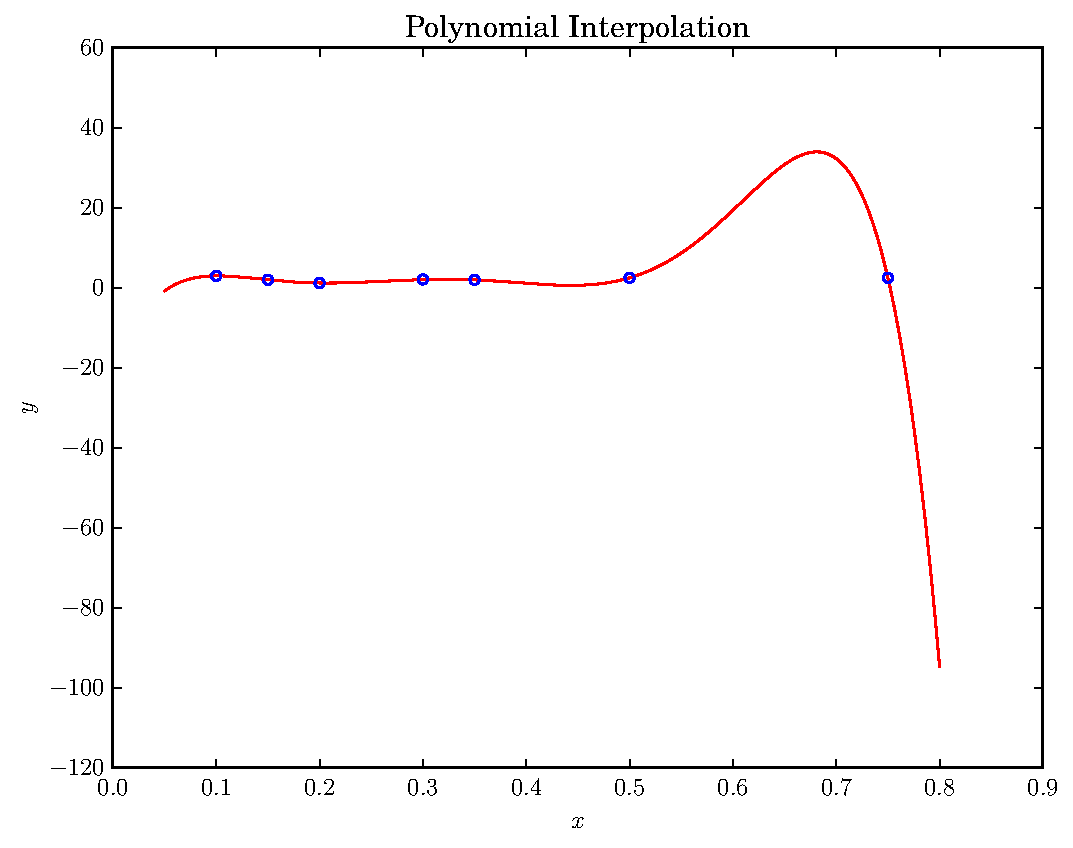
\includegraphics[width=.75\textwidth]{poly_plot.pdf}
\caption{Polynomial Interpolation. Chose $n = 6$ since there were 7 points}
\end{figure}

  \item Cubic Spline Interpolant

  {\bf Solution:}

\begin{figure}[H]
\centering
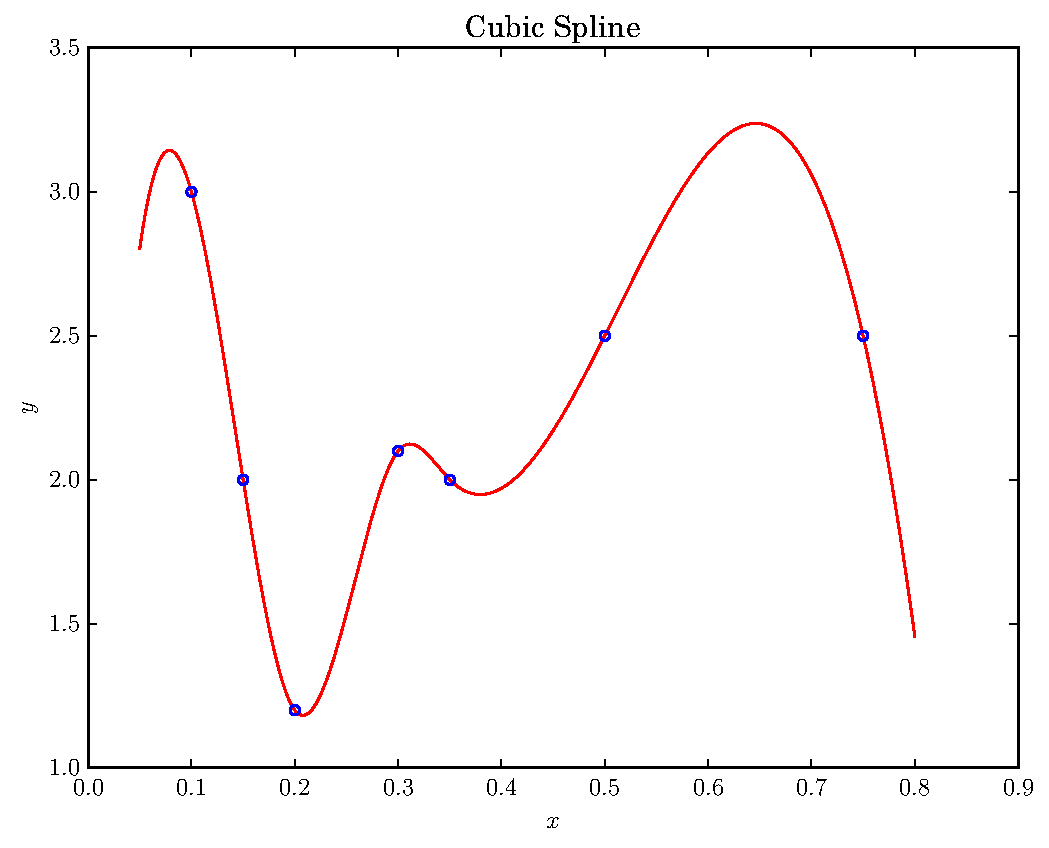
\includegraphics[width=.75\textwidth]{cubic_plot.pdf}
\caption{Cubic Spline Interpolation using {\tt scipy.interpolate.UnivariateSpline}}
\end{figure}

  \item The Interpolant

  \[
      v(x) = \sum_{j=0}^{n}c_{j}\phi_{j}(x)
  \]

  where $n = 7$, $\phi_{0}(x) = 1$, and

  \[
      \phi_{j}(x) = \sqrt{\left( x - x_{j-1}\right)^{2} + \epsilon^{2}} - \epsilon
  \]

  In addition to the $n$ interpolation requirements, the condition $c_{0} = -\sum_{j=1}^{n}c_{j}$
  is imposed. Construct this interpolant with
    \begin{enumerate}
      \item $\epsilon = 0.1$

      \item $\epsilon = 0.01$

      \item $\epsilon = 0.001$
    \end{enumerate}

  Make as many observations as you can. What will happen if we let $\epsilon \rightarrow 0$?

  {\bf Solution:}

\begin{figure}[H]
\centering
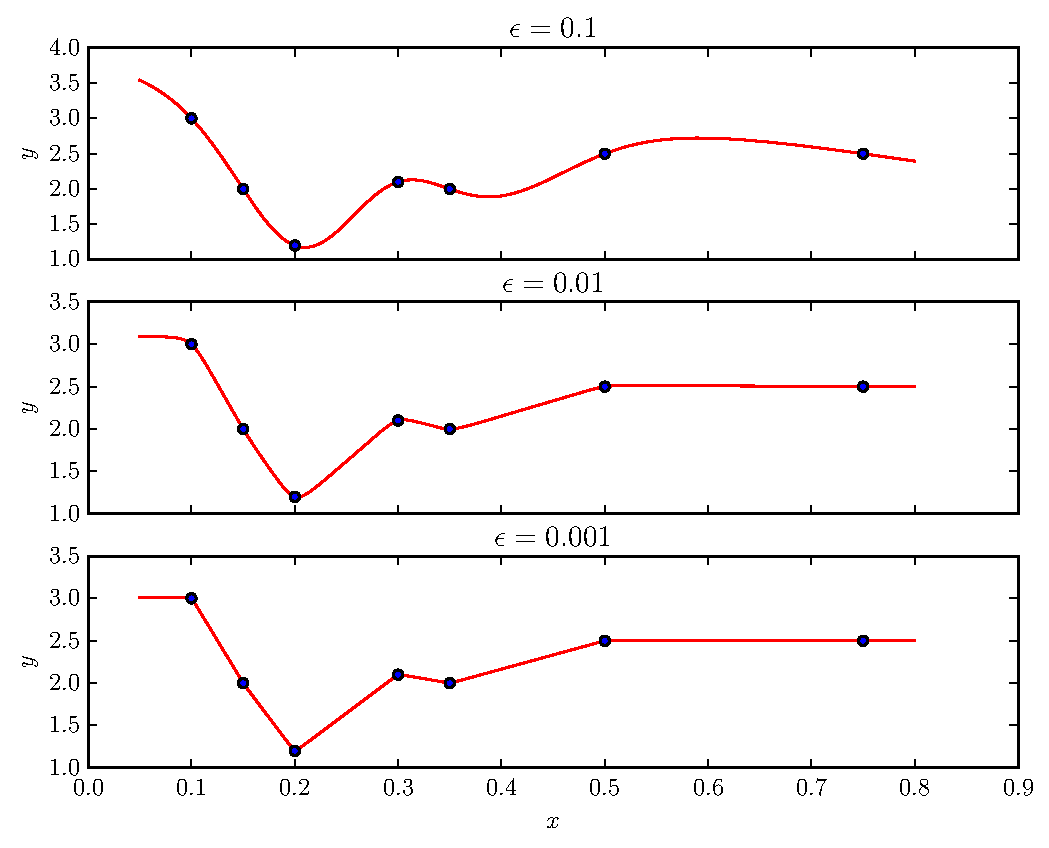
\includegraphics[width=.75\textwidth]{int_plot.pdf}
\caption{Interpolation based on the given function for different values of $\epsilon$}
\end{figure}

As the value of $\epsilon$ decreased, the interpolation function became more linear. As you increase $\epsilon$, the graph smooths out.


\end{enumerate}

\end{enumerate}

%\begin{proof}
%Blah, blah, blah.  Here is an example of the \texttt{align} environment:
%Note 1: The * tells LaTeX not to number the lines.  If you remove the *, be sure to remove it below, too.
%Note 2: Inside the align environment, you do not want to use $-signs.  The reason for this is that this is already a math environment. This is why we have to include \text{} around any text inside the align environment.
%\begin{align*}
%\sum_{i=1}^{k+1}i & = \left(\sum_{i=1}^{k}i\right) +(k+1)\\
%& = \frac{k(k+1)}{2}+k+1 & (\text{by inductive hypothesis})\\
%& = \frac{k(k+1)+2(k+1)}{2}\\
%& = \frac{(k+1)(k+2)}{2}\\
%& = \frac{(k+1)((k+1)+1)}{2}.
%\end{align*}
%\end{proof}

\end{document}
